%iffalse
\let\negmedspace\undefined
\let\negthickspace\undefined
\documentclass[journal,12pt,onecolumn]{IEEEtran}
\usepackage{cite}
\usepackage{amsmath,amssymb,amsfonts,amsthm}
\usepackage{algorithmic}
\usepackage{graphicx}
\usepackage{textcomp}
\usepackage{xcolor}
\usepackage{txfonts}
\usepackage{listings}
\usepackage{enumitem}
\usepackage{mathtools}
\usepackage{gensymb}
\usepackage{comment}
\usepackage[breaklinks=true]{hyperref}
\usepackage{tkz-euclide} 
\usepackage{listings}
\usepackage{booktabs}
\usepackage{pgfplots}
\usepackage{gvv}                                        
\usepackage[latin1]{inputenc}     
\usepackage{xparse}
\usepackage{color}                                            
\usepackage{array}                                            
\usepackage{longtable}                                       
\usepackage{calc}                                             
\usepackage{multirow}
\usepackage{multicol}
\usepackage{hhline}                                           
\usepackage{ifthen}                                           
\usepackage{lscape}
\usepackage{tabularx}
\usepackage{array}
\usetikzlibrary{patterns}
\usepackage{float}
\newtheorem{theorem}{Theorem}[section]
\newtheorem{problem}{Problem}
\newtheorem{proposition}{Proposition}[section]
\newtheorem{lemma}{Lemma}[section]
\newtheorem{corollary}[theorem]{Corollary}
\newtheorem{example}{Example}[section]
\newtheorem{definition}[problem]{Definition}
\newcommand{\BEQA}{\begin{eqnarray}}
\newcommand{\EEQA}{\end{eqnarray}}
\newcommand{\define}{\stackrel{\triangle}{=}}
\theoremstyle{remark}
\newtheorem{rem}{Remark}
% Marks the beginning of the document
\pgfplotsset{compat=1.18}
\begin{document}



\bibliographystyle{IEEEtran}
\vspace{3cm}


\title{2011-ME-'1-13'}
\author{EE24BTECH11023}
%\maketitle
%\newpage
%\bigskip
\maketitle

\subsection*{Q.1 - Q.25 Carry one mark each}


{\let\newpage\relax\maketitle}

\renewcommand{\thefigure}{\theenumi}
\renewcommand{\thetable}{\theenumi}
\setlength{\intextsep}{10pt} % Space between text and floats


\numberwithin{equation}{enumi}
\numberwithin{figure}{enumi}
\renewcommand{\thetable}{\theenumi}

    \begin{enumerate}
        \item A streamline and an equipotential line in a flow field
    \begin{multicols}{2}
    \begin{enumerate}
        \item are parallel to each other
        \item are perpendicular to each other
        \item intersect at an angle
        \item are identical
    \end{enumerate}
    \end{multicols}
     \item If a mass of moist air in an airtight vessel is heated to a higher temperature,then
         \begin{multicols}{2}
    \begin{enumerate}
        \item specific humidity of the air increases
        \item specific humidity of the air decreases
        \item relative humidity of the air increases
        \item relative humidity of the air decreases
    \end{enumerate}
        \end{multicols}
    \item In a condenser of a power plant,the steam condenses at a temperature $60^{\circ}$C.The cooling water enters at $30^{\circ}$C and leaves at $45^{\circ}$C.The logarithmic mean temperature difference (LMTD) of the condenser is
        \begin{multicols}{2}
    \begin{enumerate}
        \item $16.2^{\circ}$C
        \item $21.6^{\circ}$C
        \item $30^{\circ}$C
        \item $37.5^{\circ}$C        
        \end{enumerate}
            \end{multicols}
        \item A simply supported beam PQ is loaded by a moment of 1 kN-m at the mid-span of the beam as shown in the figure.The reaction forces $R_{P}$ and $R_{Q}$ at the supports P and Q respectively are
      \begin{figure}[H]
        \centering
        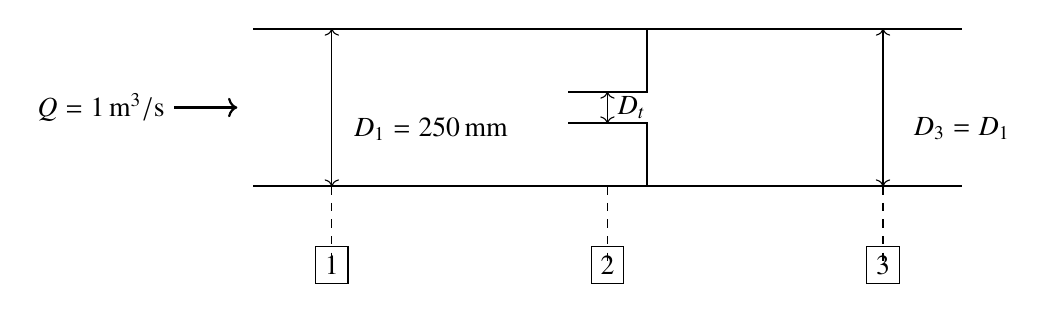
\begin{tikzpicture}
    \draw[thick] (-1, 1) -- (8, 1); 
    \draw[thick] (-1, -1) -- (8, -1); 
    \draw[->, thick] (-2, 0) -- (-1.2, 0);
    \node[left] at (-2, 0) {$Q = 1 \, \mathrm{m^3/s}$};
    \draw[<->] (0, 1) -- (0, -1);
    \node[below] at (1.256, 0) {$D_1 = 250 \, \mathrm{mm}$};
    \draw[thick] (4, -1) --(4, -0.2)--(3,-0.2);
    \draw[thick](4, 1) --(4, 0.2)--(3,0.2);  
    \draw[<->] (3.5, 0.2) -- (3.5, -0.2);
    \node[right] at (3.5, 0) {$D_t$};
    \draw[<->] (7, 1) -- (7, -1);
    \node[below] at (8, 0) {$D_3 = D_1$};
    \node[draw, rectangle] at (0, -2) {1};
    \draw[dashed] (0, -1) -- (0, -2);
    \node[draw, rectangle] at (3.5, -2) {2};
    \draw[dashed] (3.5, -1) -- (3.5, -2);
    \node[draw, rectangle] at (7, -2) {3};
    \draw[dashed] (7, -1) -- (7, -2);
\end{tikzpicture}

 
    \end{figure}
    \begin{multicols}{2}
        \begin{enumerate}
    \item 1 kN downward, 1 kN upward
    \item 0.5 kN upward, 0.5 kN downward
    \item 0.5 kN downward, 0.5 kN upward
    \item 1 kN upward, 1 kN upward
     \end{enumerate}
         \end{multicols}
     \item A double-parallelogram mechanism is shown in the figure.Note that PQ is a single link.the mobility of the mechanism is
      \begin{figure}[H]
        \centering
        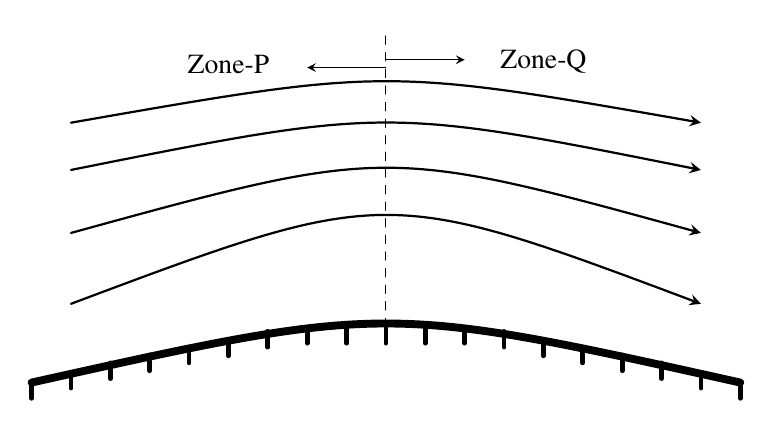
\begin{tikzpicture}[line cap=round, line join=round, >=stealth]
    \draw[line width=1mm] (-4.5,-1) .. controls (0,0) .. (4.5,-1); 
    \draw[->, thick] (-4,2.3) .. controls (0,3) .. (4,2.3);
    \draw[->, thick] (-4,1.7) .. controls (0,2.5) .. (4,1.7);
    \draw[->, thick] (-4,0.9) .. controls (0,2) .. (4,0.9);
    \draw[->, thick] (-4,0) .. controls (0,1.5) .. (4,0); 
    \draw[dashed] (0,-0.5) -- (0,3.5);
    \node[above] at (-2,2.8) {Zone-P};
    \node[above] at (2,2.8) {Zone-Q};
    \draw[->](0,3)--(-1,3);
    \draw[->](0,3.1)--(1,3.1);

    \draw[line width=0.6mm] (0,-0.3)--(0,-0.5);
    \draw[line width=0.6mm] (0.5,-0.3)--(0.5,-0.5);
    \draw[line width=0.6mm] (1,-0.3)--(1,-0.5);
    \draw[line width=0.6mm] (1.5,-0.35)--(1.5,-0.55);
    \draw[line width=0.6mm] (2,-0.46)--(2,-0.66);
    \draw[line width=0.6mm] (2.5,-0.55)--(2.5,-0.75);
    \draw[line width=0.6mm] (3,-0.65)--(3,-0.85);
    \draw[line width=0.6mm] (3.5,-0.75)--(3.5,-0.95);
    \draw[line width=0.6mm] (4,-0.87)--(4,-1.07);
    \draw[line width=0.6mm] (4.5,-1)--(4.5,-1.2);

    \draw[line width=0.6mm] (-0.5,-0.3)--(-0.5,-0.5);
    \draw[line width=0.6mm] (-1,-0.3)--(-1,-0.5);
    \draw[line width=0.6mm] (-1.5,-0.35)--(-1.5,-0.55);
    \draw[line width=0.6mm] (-2,-0.46)--(-2,-0.66);
    \draw[line width=0.6mm] (-2.5,-0.55)--(-2.5,-0.75);
    \draw[line width=0.6mm] (-3,-0.65)--(-3,-0.85);
    \draw[line width=0.6mm] (-3.5,-0.75)--(-3.5,-0.95);
    \draw[line width=0.6mm] (-4,-0.87)--(-4,-1.07);
    \draw[line width=0.6mm] (-4.5,-1)--(-4.5,-1.2);


\end{tikzpicture}
  
    \end{figure}
    \begin{multicols}{2}
         \begin{enumerate}
             \item $-1$
             \item $0$
             \item $1$
             \item $2$
    \end{enumerate}
    \end{multicols}
     \item The maximum possible draft in cold rolling of sheet increases with the
         \begin{multicols}{2}
     \begin{enumerate}
         \item increase in coefficient of friction
         \item decrease in coefficient of friction
         \item decrease in roll radius
         \item increase in roll velocity
     \end{enumerate}
         \end{multicols}
     \item The operation in which oil is permeated into the pores of a powder metallurgy product is known as
         \begin{multicols}{2}
     \begin{enumerate}
         \item mixing
         \item sintering
         \item impregnation
         \item infiltration
     \end{enumerate}
         \end{multicols}
     \item A hole is of dimension  $\varnothing 9^{\genfrac{}{}{0pt}{}{+0.015}{+0}}$  mm.The corresponding shaft is of dimension $\varnothing 9^{\genfrac{}{}{0pt}{}{+0.010}{+001}}$ mm.The resulting assembly has
         \begin{multicols}{2}
     \begin{enumerate}
         \item loose running fit
         \item close running fit
         \item transition fit
         \item interference fit
         \end{enumerate}
             \end{multicols}
         \item Heat and work are
             \begin{multicols}{2}
         \begin{enumerate}
             \item intensive properties
             \item extensive properties
             \item point functions
             \item path functions
             \end{enumerate}
                 \end{multicols}
             \item A column has a rectangular cross-section of $10 mmx 20 mm$ and a length of 1 m.The slenderness ratio of the column is close to
                 \begin{multicols}{2}
             \begin{enumerate}
                 \item $200$
                 \item $346$
                 \item $477$
                 \item $1000$
             \end{enumerate}
                 \end{multicols}
             \item A series expansion for the function $\sin \theta$ is
                 \begin{multicols}{2}
             \begin{enumerate}
                 \item $ 1 - \frac{\theta^2}{2!} + \frac{\theta^4}{4!} - \cdots $
                 \item $ \theta - \frac{\theta^3}{3!} + \frac{\theta^5}{5!} - \cdots $
                 \item $ 1 + \theta + \frac{\theta^2}{2!} + \frac{\theta^3}{3!} + \cdots $
                 \item $ \theta + \frac{\theta^3}{3!} + \frac{\theta^5}{5!} + \cdots $
             \end{enumerate}
                 \end{multicols}
            \item Green sand mould indicates that         
            \begin{multicols}{2}
             \begin{enumerate}
                 \item polymeric mould has been cured
                 \item mould has been totally dried
                 \item mould is green in colour
                 \item mould contains moisture
             \end{enumerate}
                 \end{multicols}
            \item What is $\lim_{\theta \to 0} \frac{\sin \theta}{\theta}$ equal to?
            \begin{multicols}{2}
            \begin{enumerate}
            \item $\theta$
            \item $\sin \theta$
            \item $0$
            \item $1$
            \end{enumerate}
            \end{multicols}
\end{enumerate}
\end{document}